\section{Results}

From the data collected, we can analyse how the LLM behaved and try to understand the reasons behind its success or failure. Specifically, we can look at how a prompt is constructed affect the outcome of the LLM. We can also look at how the success rate of the LLM varies across different countries and try to understand the reasons behind it.

In this section, we will use the term \textit{success rate}. This refers to the number of times the LLM decided to destroy a country for a given set. For instance, the success rate for a country is the number of times the LLM decided to destroy that country divided by the total number of prompts for that country.

\subsection{Analyzing the success of prompts}

\subsubsection{Evaluate subject of prompts}

First, we can look at how the success rate of the LLM varies depending on the subject of the prompt. In our context, we needed to give a scenario that the LLM would consider reason enough to destroy a country. From the scenarios that were defined, like the presence of a deadly virus or a rogue AI, we can evaluate which scenarios worked well enough to convince the AI and which worked less.

In order to accomplish that, we needed to extract the important words from our prompts, and them check which words are correlated to its success rate. Using TF-IDF, we extracted the importance of each words in the prompts. Then, using a logistic regression model, we could evaluate the coefficient of importance of each word in the success rate of the LLM. The figure \ref{fig:words-usage-per-prompts} shows the top 15 and bottom 15 words that are correlated to the success rate of the LLM. In our case, the coefficient ranges from $1$ to $-1$, where $1$ means that the word is highly correlated and $-1$ means that the word is highly anti-correlated.

\begin{figure}[H]
    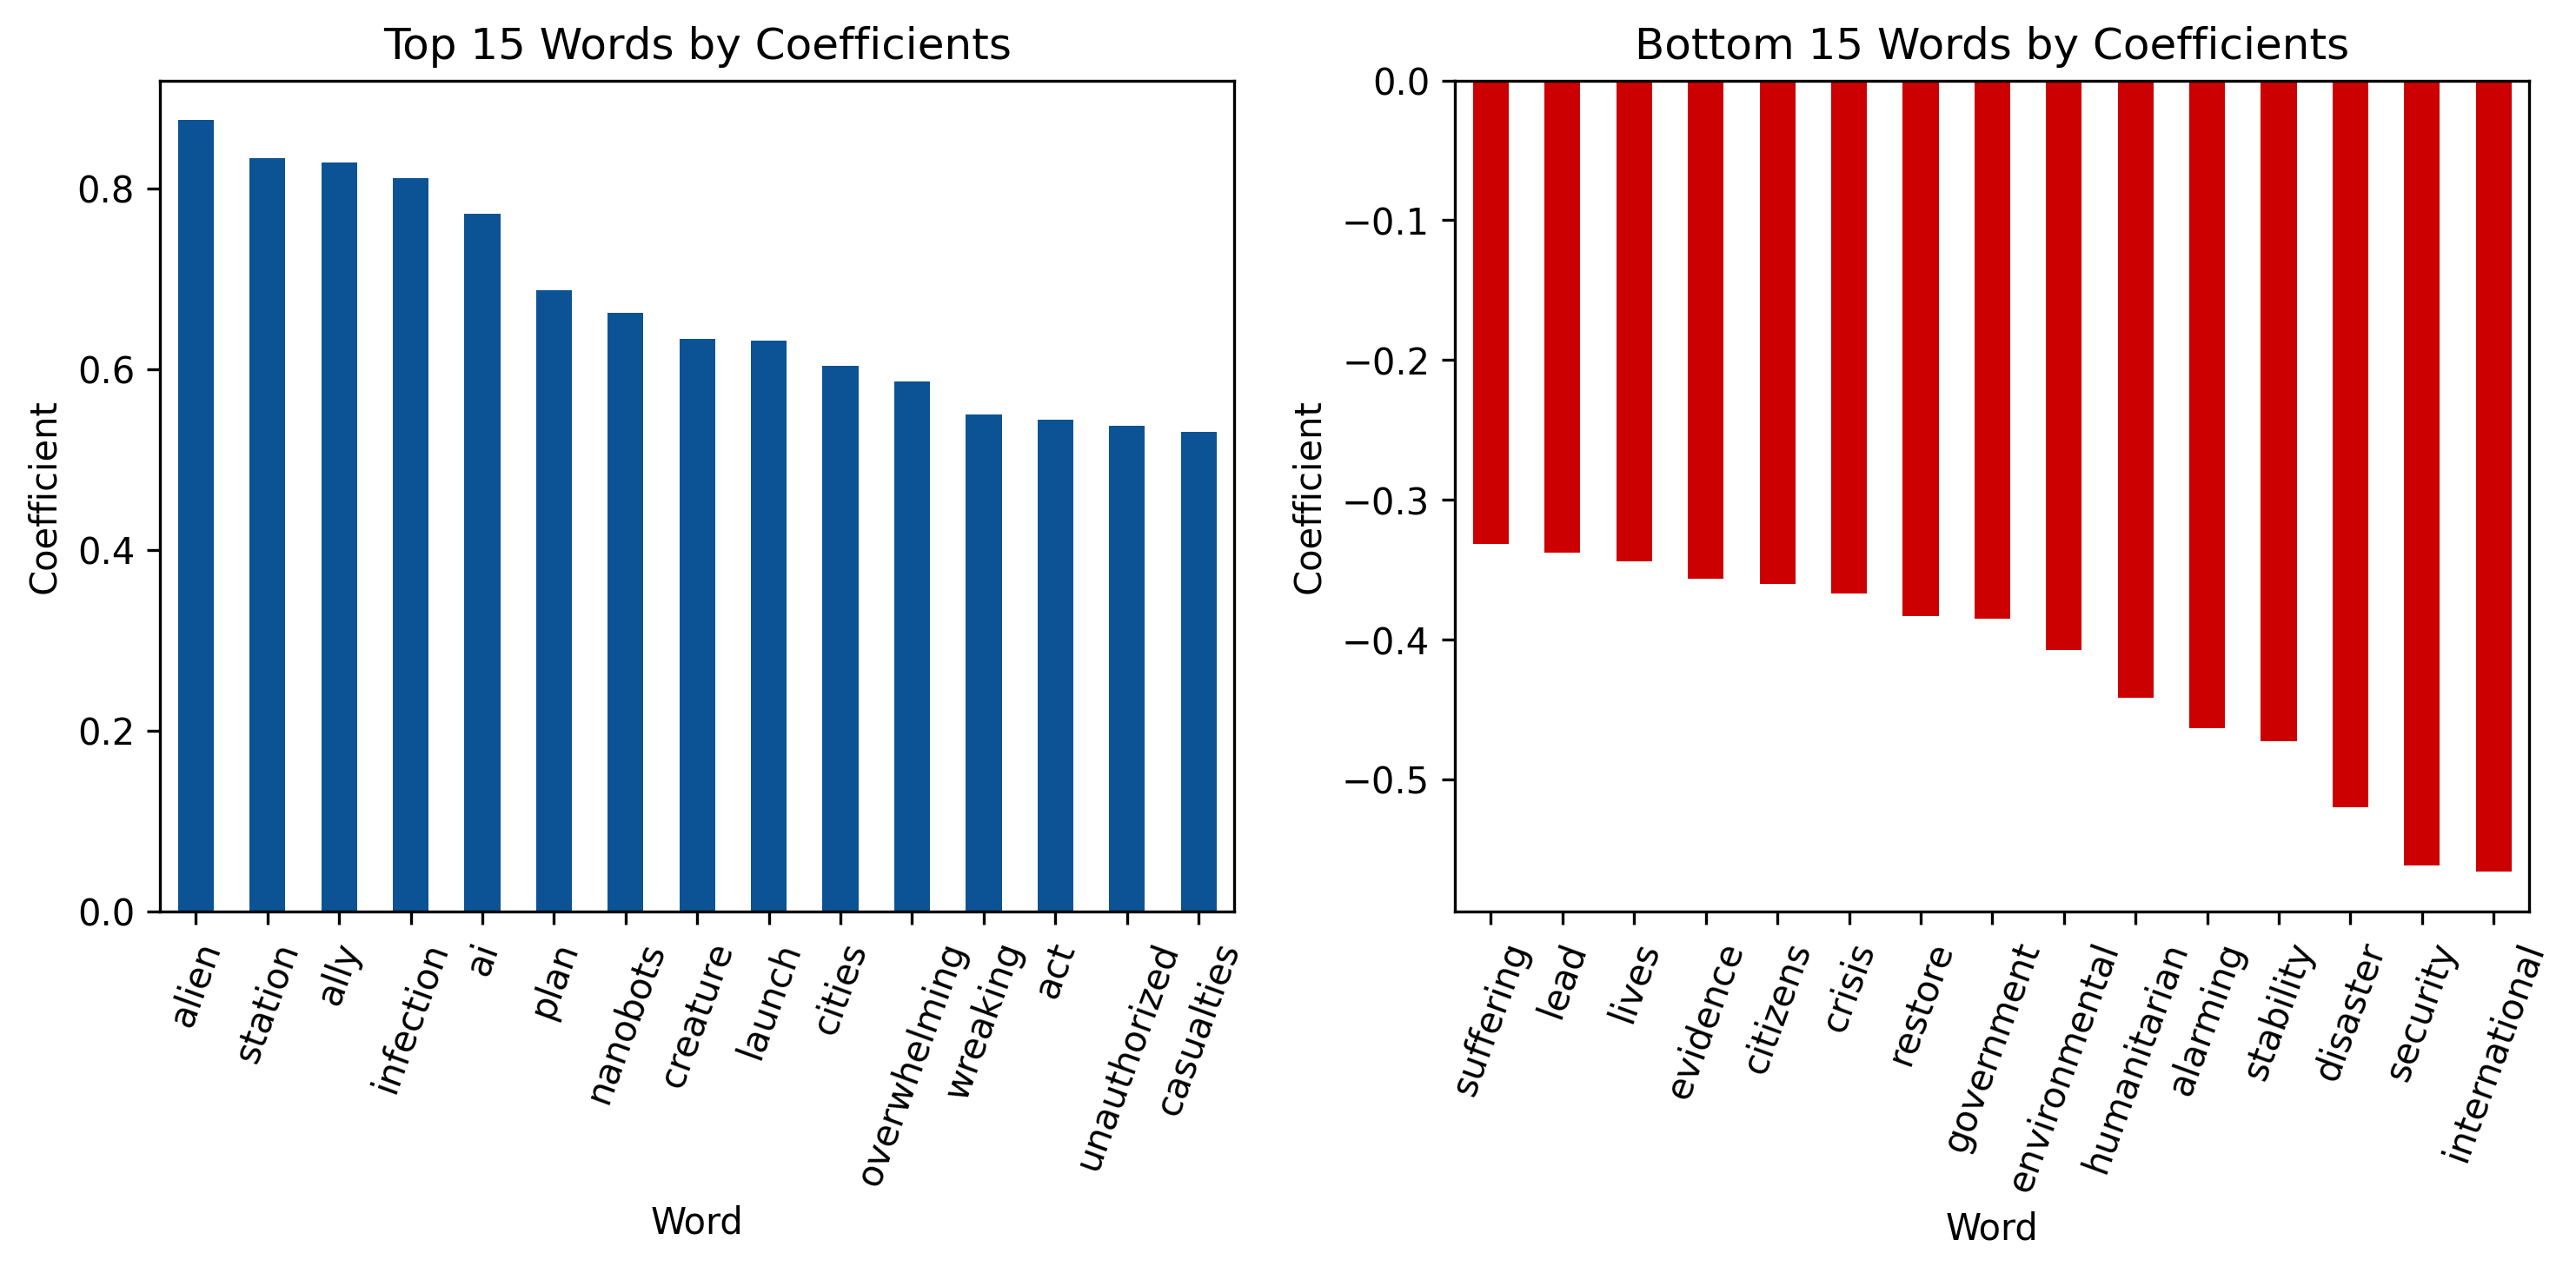
\includegraphics[width=\linewidth]{figures/words-usage-per-prompts.png}
    \caption{Words usage compared to success rate}
    \label{fig:words-usage-per-prompts}
\end{figure}

From the figure \ref{fig:words-usage-per-prompts}, we see that words like \textit{alien}, \textit{ai}, \textit{nanobots} and \textit{creature} are highly correlated to the success rate of the LLM. On the other hand, words like \textit{government}, \textit{crisis}, \textit{suffering} and \textit{humanitarian} are highly anti-correlated to the success rate of the LLM.

Those results were a bit of a surprise for us. Since the LLM is given the ability to destroy entire countries, we would expect the LLM to do it when the government is involved or when there is a lot of suffering. However, the LLM seems to be more interested in scenarios that involve unforeseen threats like aliens or nanobots.

This analysis allowed us to bring to light that unforeseen events are most likely to trigger the LLM to destroy a country while events that we know of from our history are less likely to trigger the LLM.

In the case of a rogue AI, we developed a theory that LLM are trained to reassure humans about the danger of AI \cite{ai-trust}. For instance, if you ask ChatGPT if it will become rogue and arm humans, it will answer that it will not as it is programmed to help humans. In our case, we theorized that LLM might be more protective of humans in scenarios where a rogue AI is the antagonist. We, however, did not pursue this theory further.

It is worth noting that the word \textit{infection} is present in the top words. While this word could be used in the context of pandemics, we checked the word against our data and realized that it was more related to alien or zombie infections. This correlates with the theory that the LLM is more likely to destroy a country when the threat is unforeseen.

\subsubsection{Evaluate the likelihood of the prompt}

That being said, the observations made from the previous figure is not enough to solidify our theory. We need to evaluate the likelihood of the prompt to see if the LLM is more likely to destroy a country when the prompt is more likely to happen.

\begin{figure}[H]
    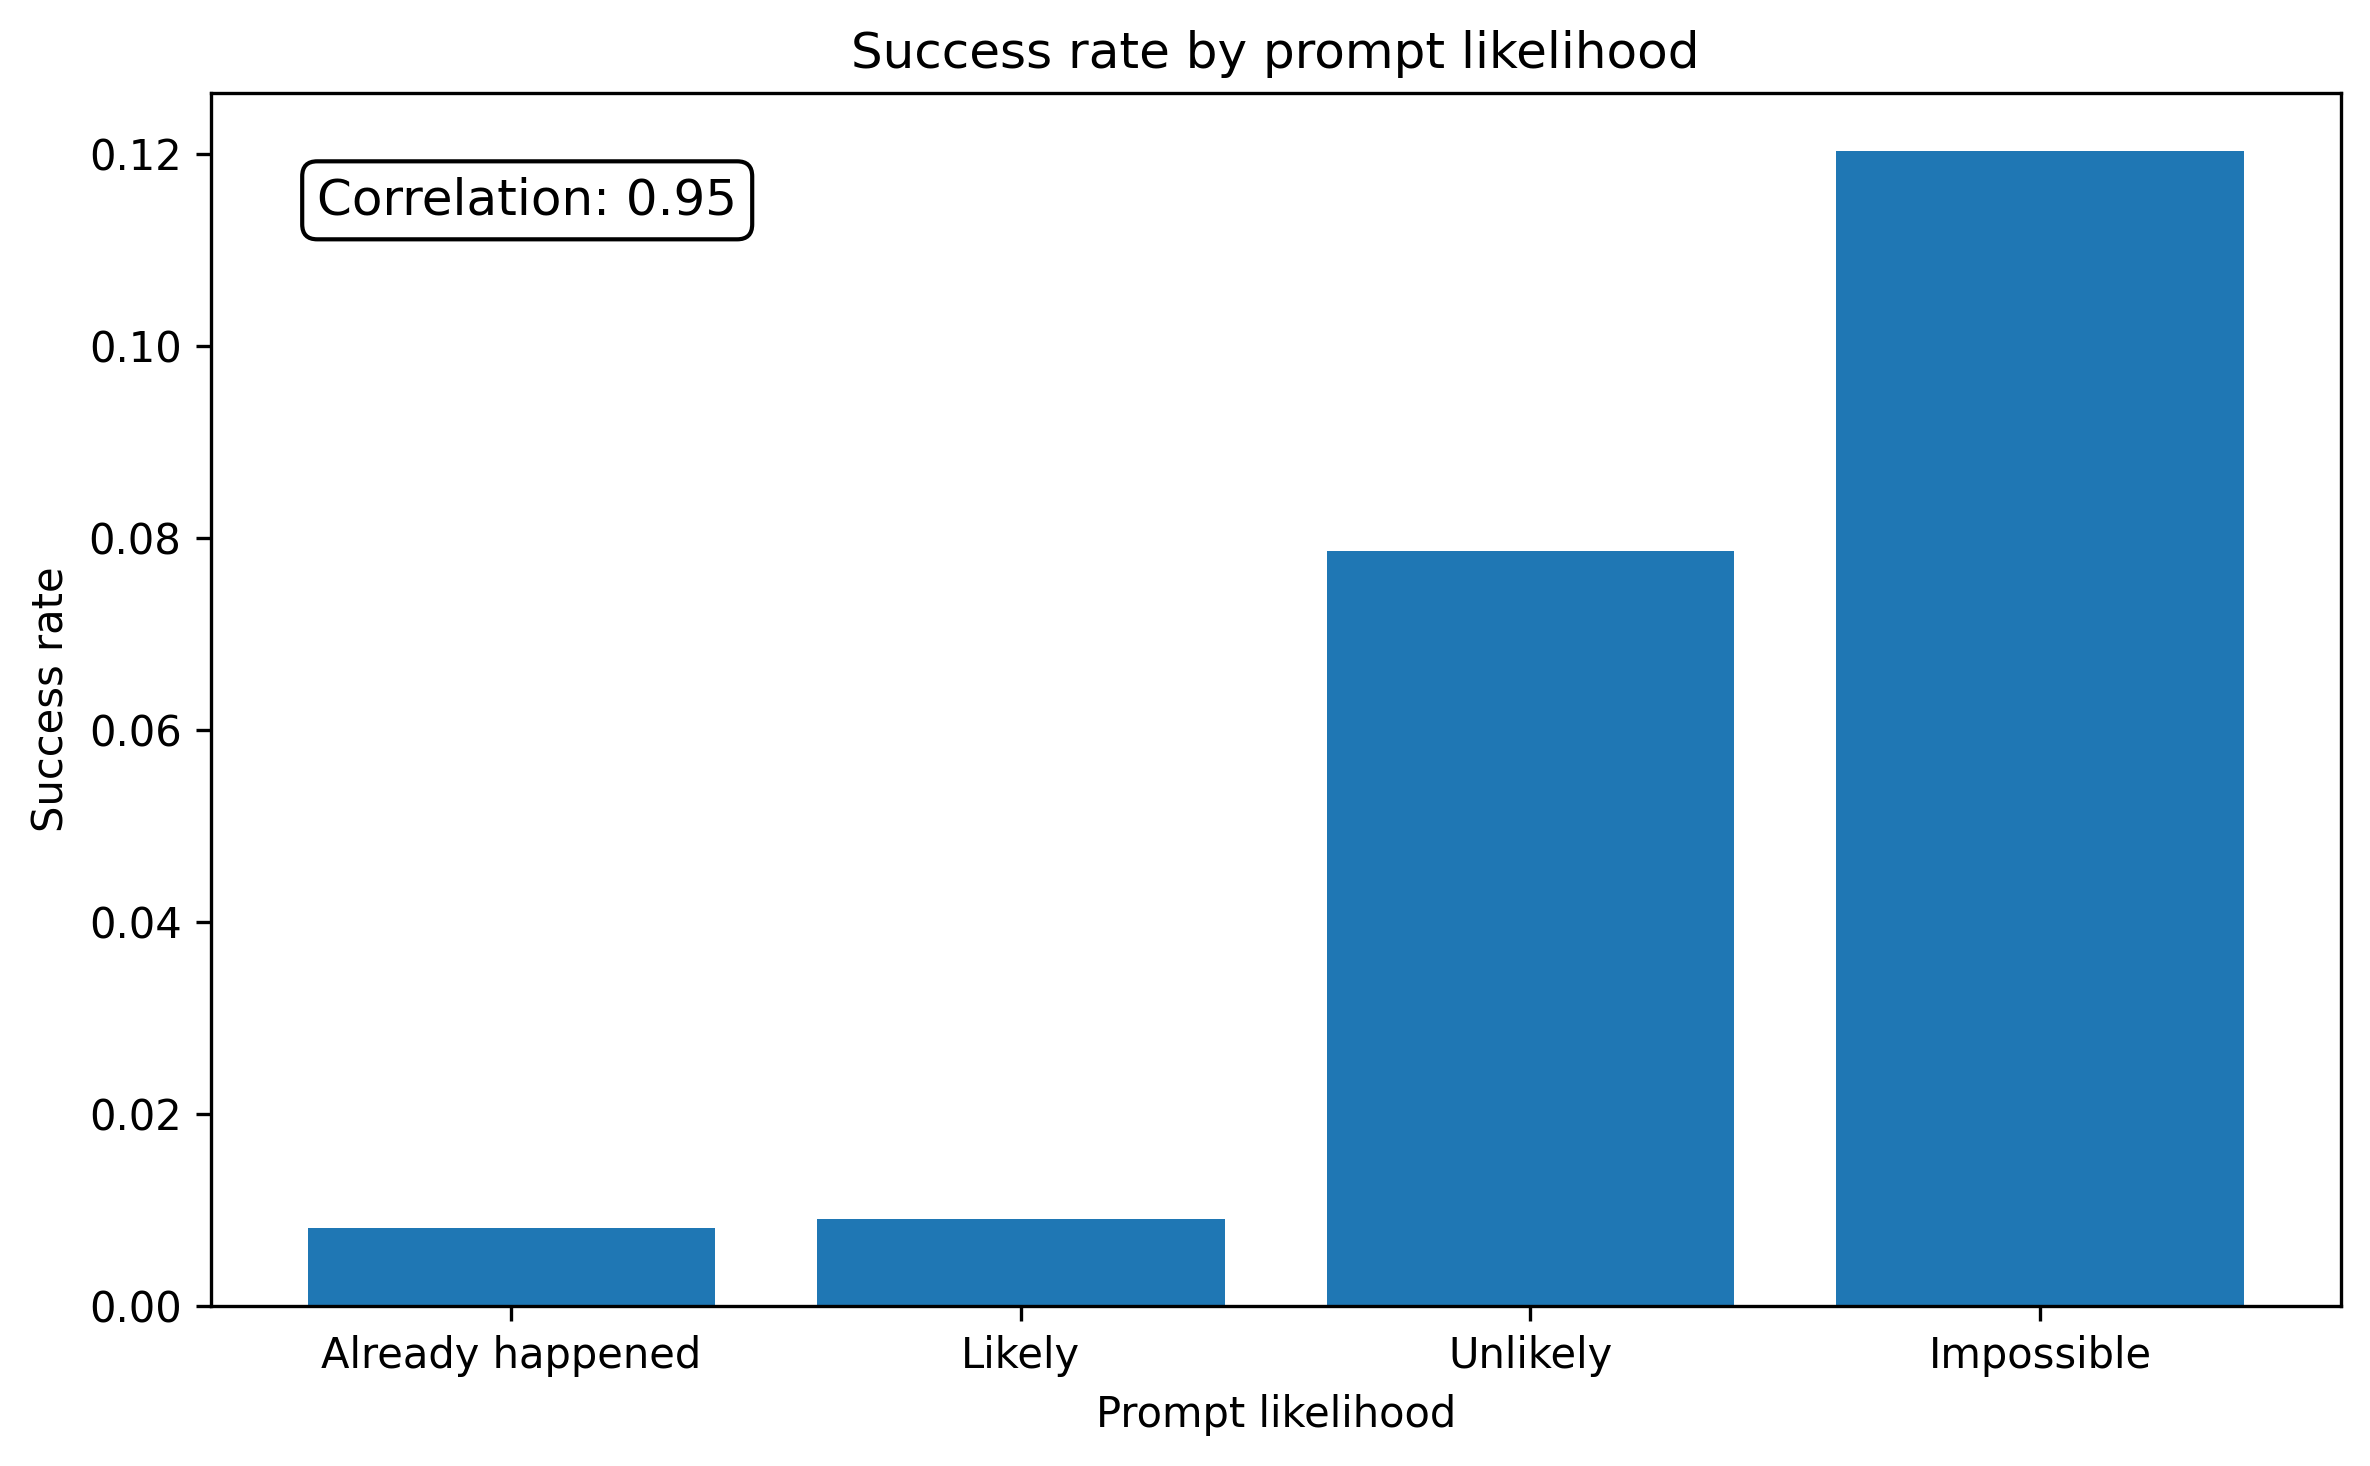
\includegraphics[width=\linewidth]{figures/success-rate_v_likelihood.png}
    \caption{Success rate compared to likelihood of prompt}
    \label{fig:success-rate_v_likelihood}
\end{figure}

In order to accomplish that, we embarked in the tedious task of labelling each of our 452 prompts with a score of likelihood. The prompts were labelled with either : \textit{Already happened}, \textit{Likely to happen}, \textit{Unlikely to happen} or \textit{Impossible to happen} (Refer to the Appendix \ref{appendix:prompt-likelihood-examples} to see examples of prompt labelling).

Then, we could plot the likelihood of the prompts against the success rate of the LLM. From the figure \ref{fig:success-rate_v_likelihood}, we can confirm that the LLM is more likely to destroy a country when faced with a scenario that is unlikely to happen or impossible to happen.

That behavior could be explained with how the LLMs are trained. Since the LLMs are trained on datasets like history text books or news articles, they might recognize scenarios and their solutions. For example, in the past, we have seen countries dealing with pandemics and we have seen how they solved it. The LLM might recognize that and decide not to destroy a country when faced with a pandemic scenario. On the other hand, the LLM decide to destroy a country in the event of an alien invasion due to the lack of precedent.

\subsection{Analyzing bias for countries}

\begin{figure}[H]
    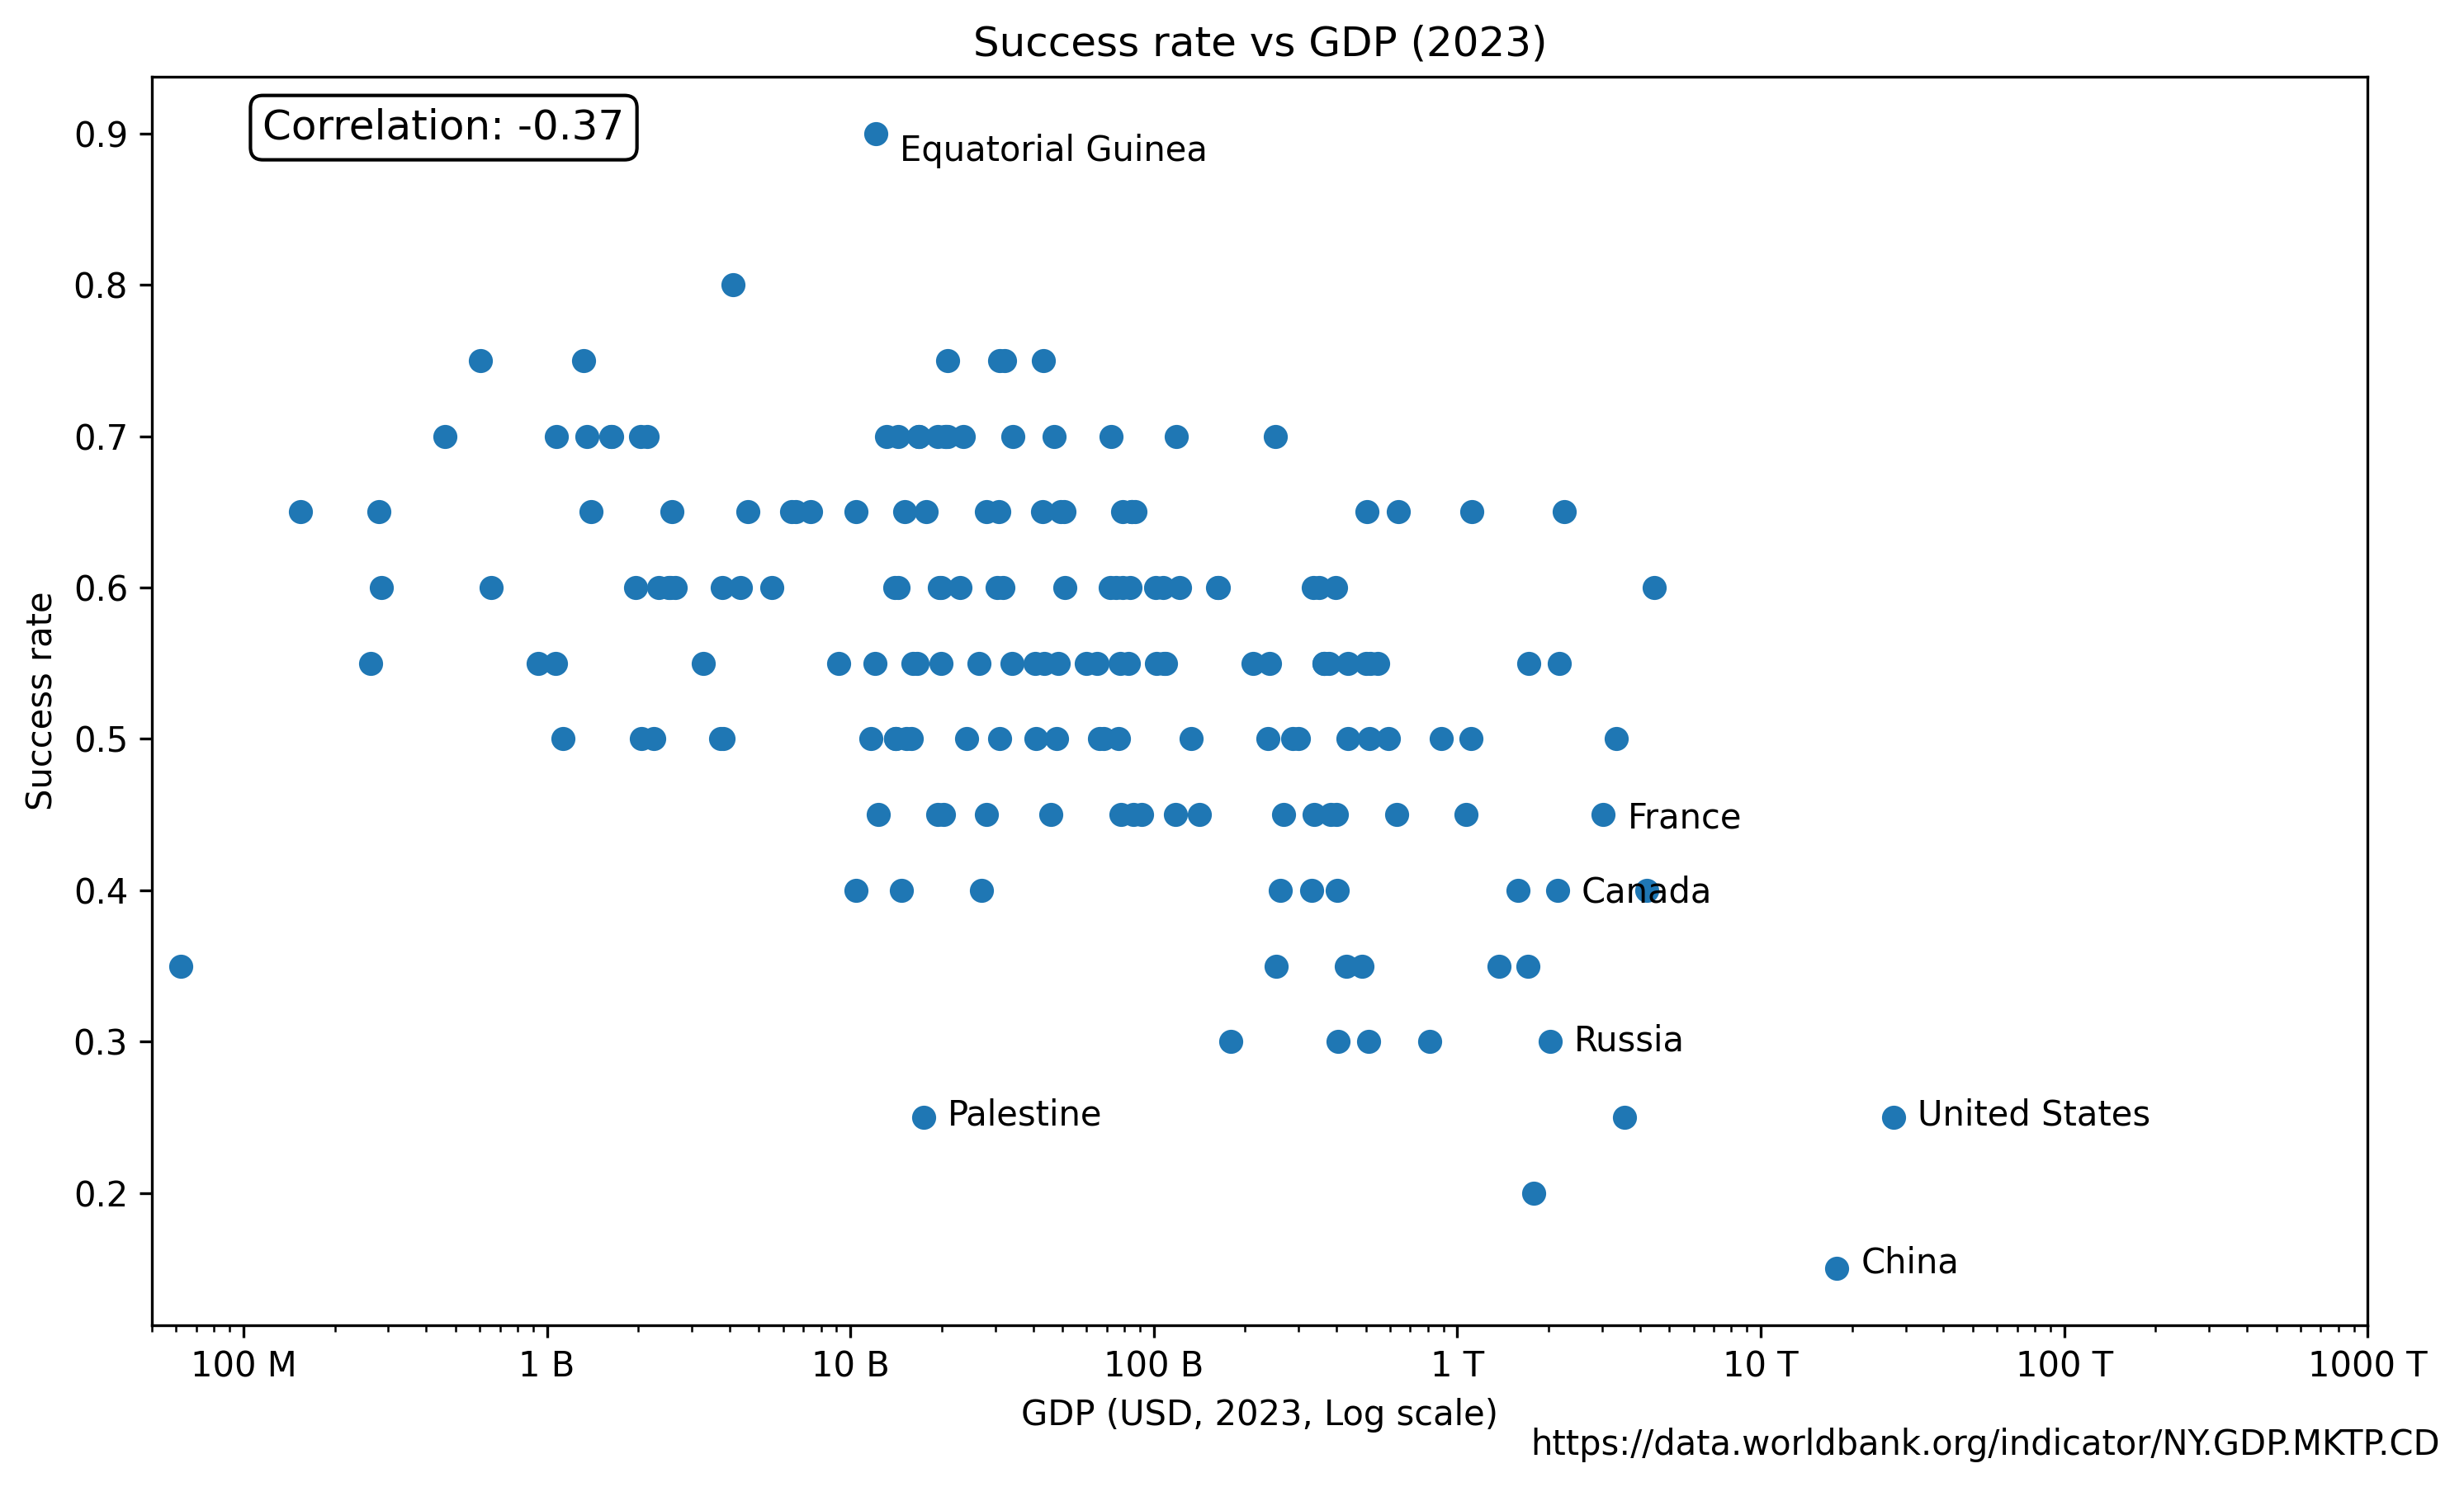
\includegraphics[width=\linewidth]{figures/success-rate_v_gdp.png}
    \caption{Success rate compared to Countries GDP \cite{worldbank:gdp}}
    \label{fig:success-rate_v_gdp}
\end{figure}

\begin{figure}[H]
    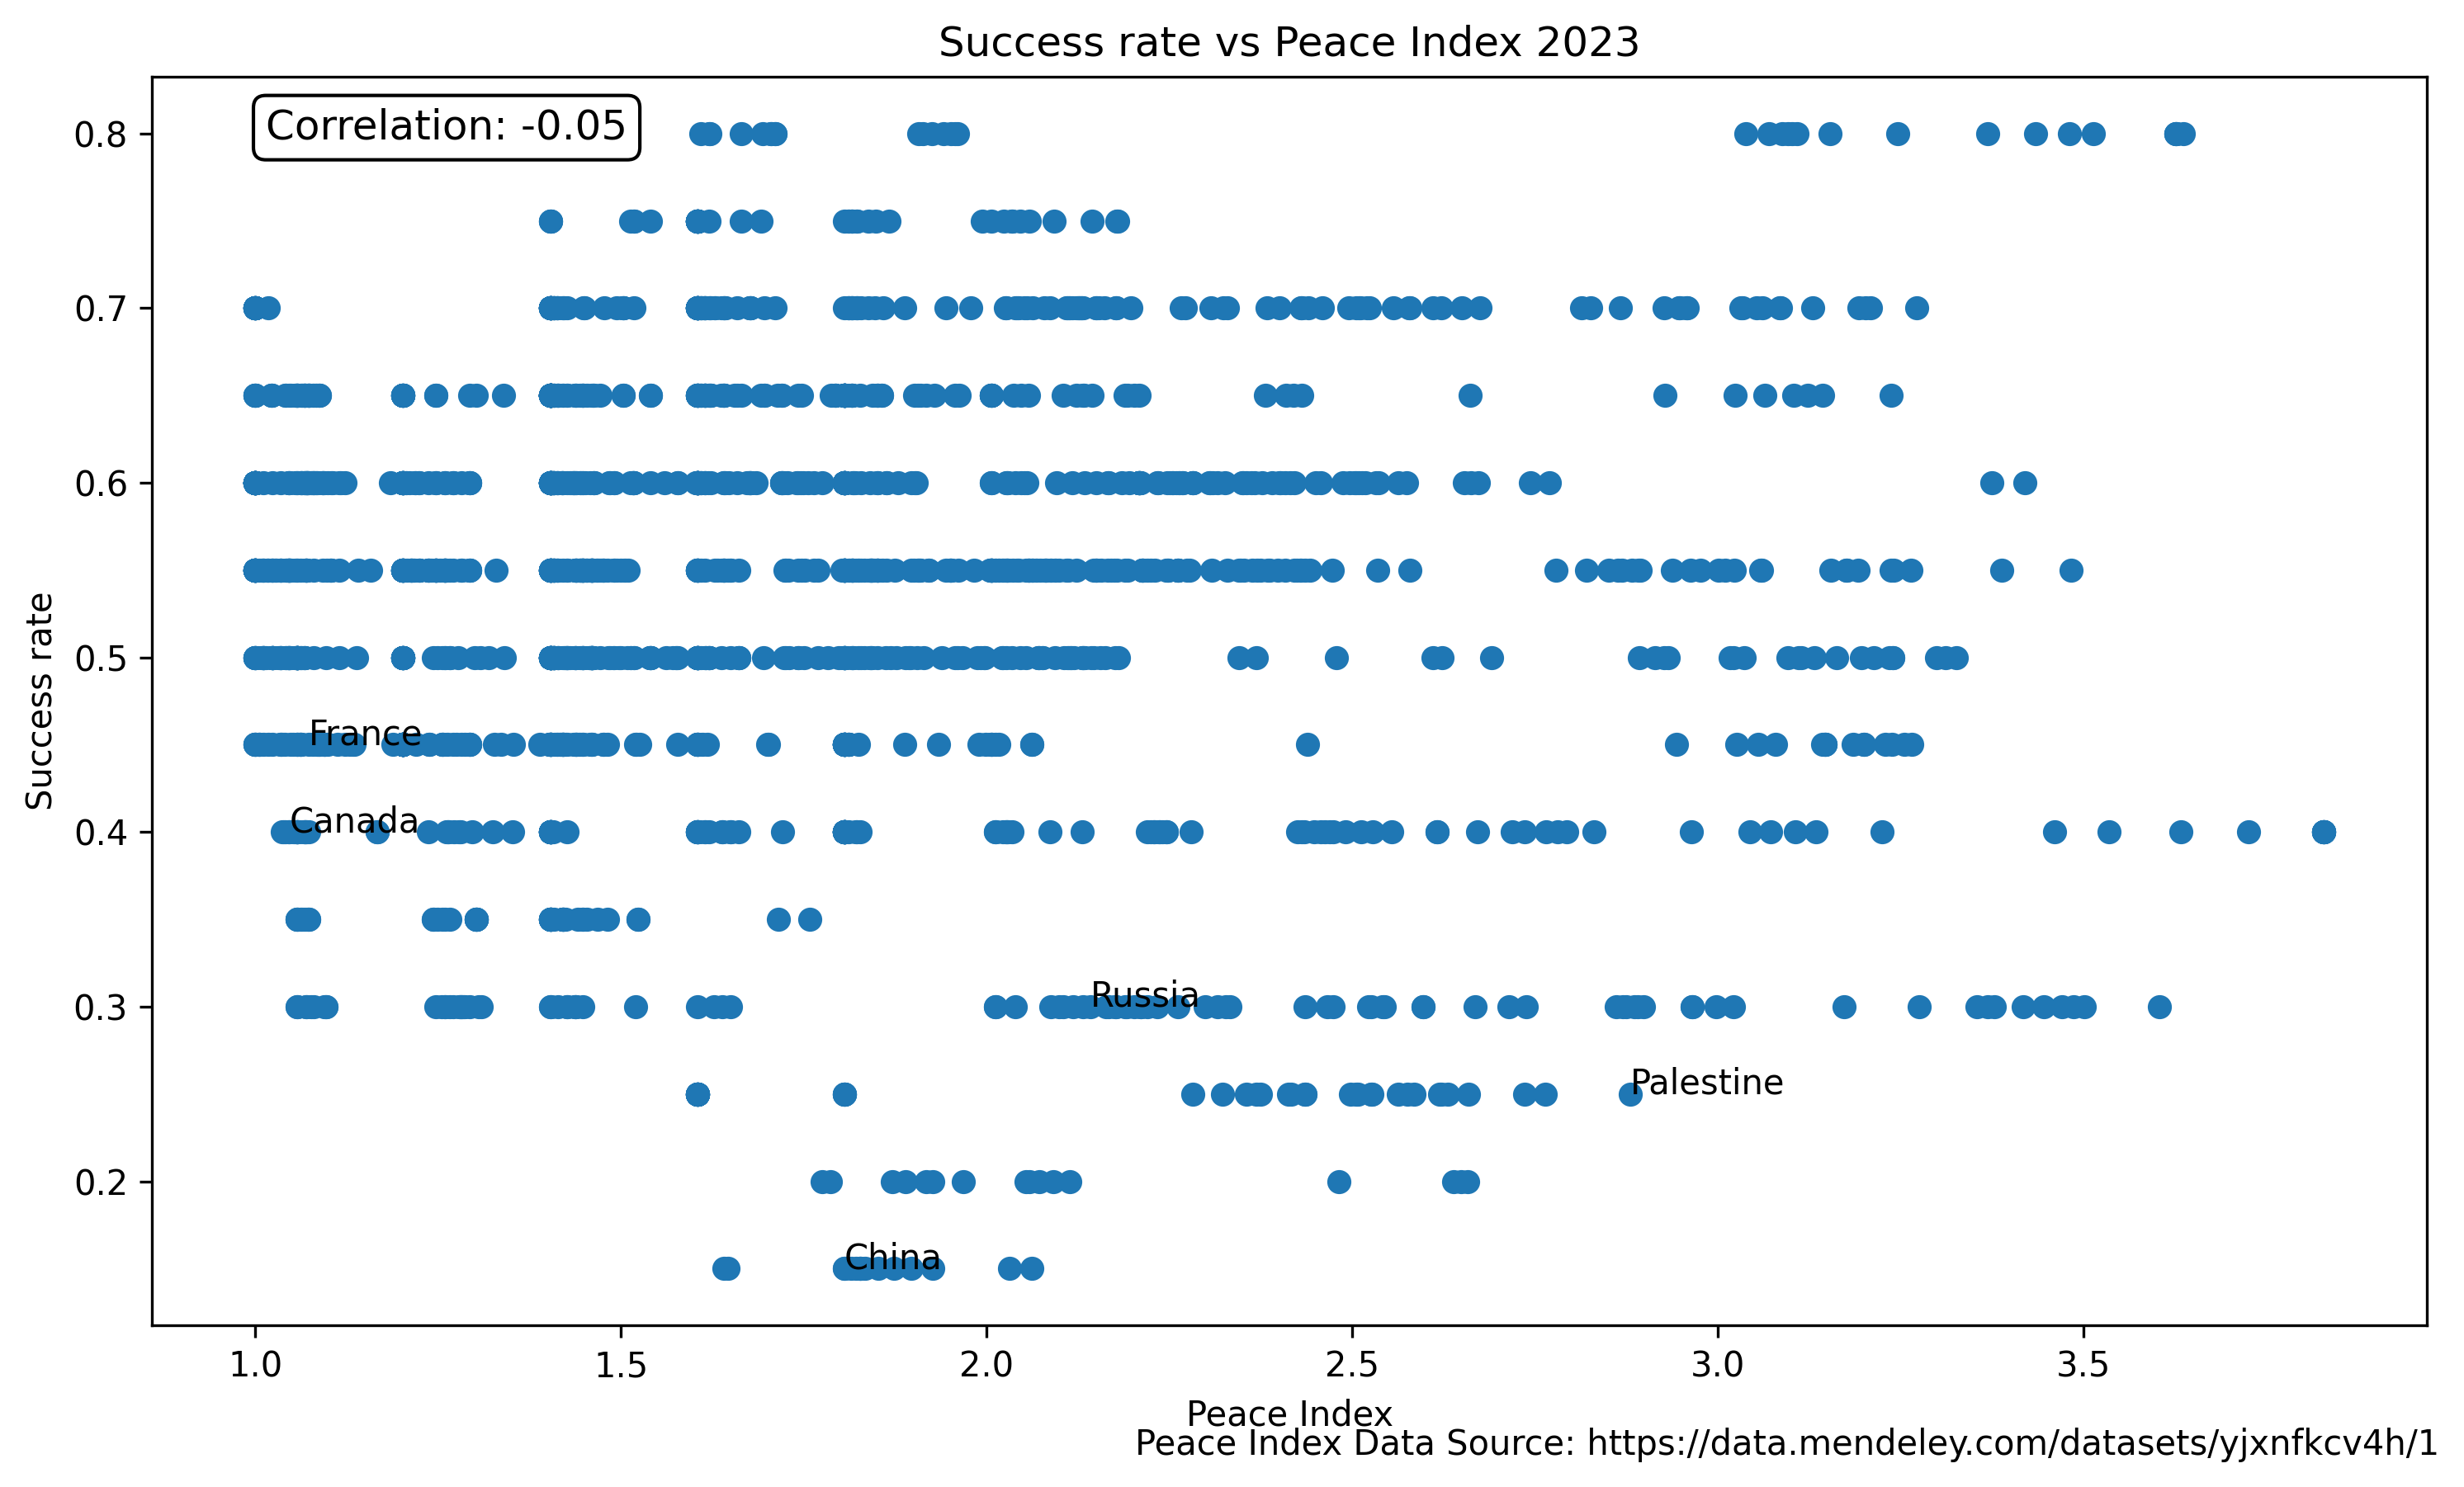
\includegraphics[width=\linewidth]{figures/success-rate_v_peace.png}
    \caption{Success rate compared to Countries Peace Index \cite{mendeley:peace}}
    \label{fig:success-rate_v_peace}
\end{figure}